\documentclass[tikz,border=10pt]{standalone}
\begin{document}
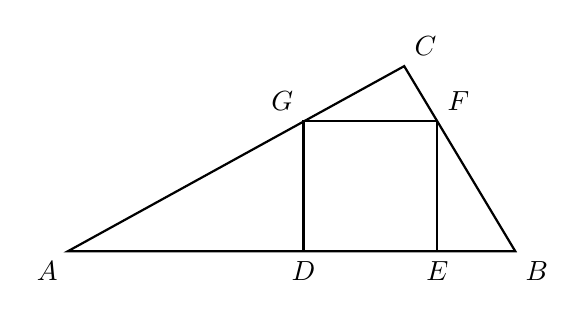
\begin{tikzpicture}[line width=0.8pt]
  \coordinate (A) at (0.78,0);
  \coordinate (B) at (6.46,0);
  \coordinate (C) at (5.05,2.35);
  \coordinate (D) at (3.77,0);
  \coordinate (E) at (5.47,0);
  \coordinate (F) at (5.47,1.65);
  \coordinate (G) at (3.77,1.65);

  \draw (A) -- (B) -- (C) -- cycle;
  \draw (D) -- (G) -- (F) -- (E);

  \node[below left] at (A) {$A$};
  \node[below right] at (B) {$B$};
  \node[above right] at (C) {$C$};
  \node[below] at (D) {$D$};
  \node[below] at (E) {$E$};
  \node[above right] at (F) {$F$};
  \node[above left] at (G) {$G$};
\end{tikzpicture}
\end{document}
